\documentclass{article}
\usepackage[T1]{fontenc}
\usepackage{lmodern}
\usepackage{graphicx}
\usepackage{amsmath,amssymb}
\usepackage[a4paper,margin=2cm]{geometry}
\usepackage[absolute,overlay]{textpos}
\setlength{\TPHorizModule}{1mm}
\setlength{\TPVertModule}{1mm}
\usepackage[indonesian]{babel}
\usepackage{hyperref}
\setlength{\emergencystretch}{2em}
% unit: Halaman 29

\begin{document}

% === Halaman 29 (llm) ===

\vspace{243.54mm}

Contoh hasil enkripsi DES pada setiap putaran:

\vspace{20mm}

Sumber: Cryptography and Network Security \\ Chapter 3, Lecture slides by Lawrie Brown \\ Modified by Richard Newman

% deskripsi: Tabel yang menunjukkan hasil enkripsi DES untuk setiap putaran, mencakup kolom Round, K_i (kunci putaran), L_i (setengah kiri), dan R_i (setengah kanan) dari tahap IP hingga IP^-1.
% bbox normalisasi: [0.2400, 0.1300, 0.7200, 0.9500]
\begin{textblock*}{100.80mm}(50.40mm,38.61mm)
\noindent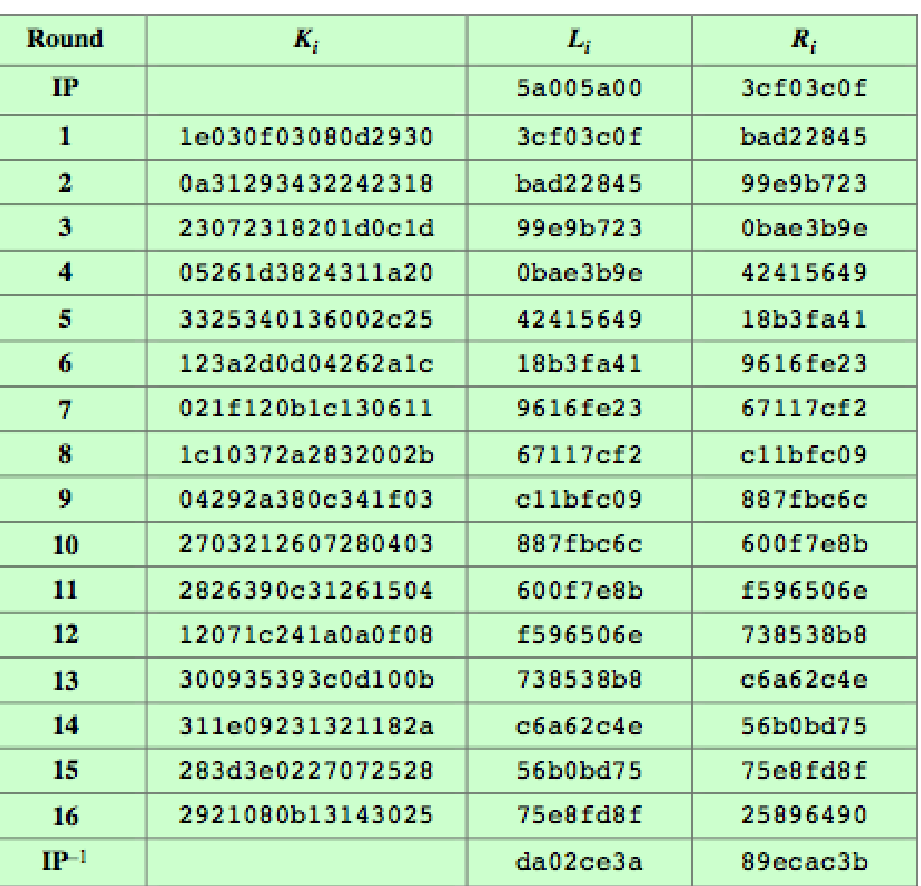
\includegraphics[width=100.80mm,height=243.54mm]{../../images/llm/page_029_img_01.png}%
\end{textblock*}

\end{document}
